\section{Security considerations}\label{sec:secure}
In order to increase the level of security in our system, different considerations should be made. These considerations are made in order to make it more difficult for intruders to break into the system as well as protect sensitive information. We limit the discussion to program communication and the way sensitive information is handled, as this is the most sensitive part of the system. It would also improve the robustness of the system if these parts were made secure, as these are the parts of the program where it is possible to introduce erroneous, dirty data.

\subsection*{Certificates}
Certificates are used when communicating over the HTTPS protocol as a way to ensure the identity of a website as well as hand out the public key and encryption method. Once a certificate for a website is downloaded to a computer, the identity of the website can be verified against this certificate on subsequent visits. All communication with MSE uses the HTTPS protcol, and as such we have to consider how we treat certificates. 

Initially we created an empty certificate-handler which is still in use. This means that the identity of a website is accepted no matter what, potentially allowing for scam websites to copy the certificate and alter it slightly to pose as another website. An alternative, more secure solution, would be to download the certificates MSE uses and insert them in the JVM keystore, which is a collection of all accepted certificates. By freely accepting all certificates it is possible for attackers to input dirty data in the system by adding a server pretending to be an MSE service.

\subsection*{HTTPS}
The system currently communicates internally over HTTP, an insecure communication protocol that uses cleartext to communicate. Anybody intercepting the communication can read it with ease. We can diminish the damage from this type of attack by using the HTTPS protocol, short for \textit{Hyper Text Transfer Protocol Secure}, which functions as the HTTP protocol with the exception that the message is encrypted. This means that if someone were to gain access to the connection, they would not be able to read the information. A secure connection is very important on sites that handle sensitive information such as CPR-numbers or credit card data and this can be achieved by using the HTTPS protocol \cite{HTTPS}.

\begin{figure}[ht]
	\begin{center}
		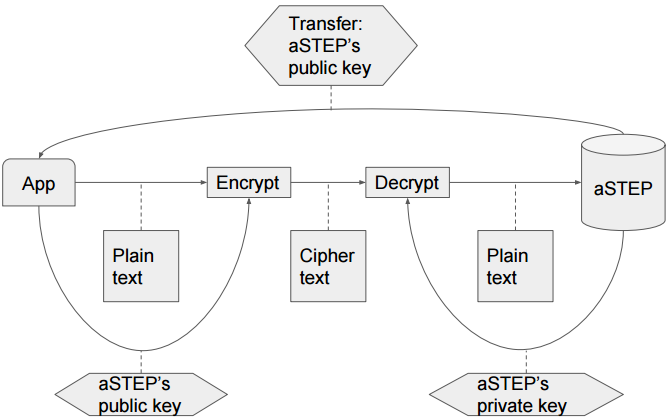
\includegraphics[scale=0.9]{graphics/encrypt_decrypt.png}
		\caption{HTTPS.}
		\label{fig:HTTPS}
	\end{center} 
\end{figure}

\Cref{fig:HTTPS} shows how HTTPS is used. In this example an app is sending data to the aSTEP server via the HTTPS protocol. First the app retrieves aSTEP's public key from the downloaded certificate. This public key is then used to encrypt all the data that is going to be sent to aSTEP. When aSTEP receives the data, the private key is used to decrypt the data, which can then be read as plain text. Additionally, if aSTEP needs to send data back to the app, it will need the apps public key to encrypt the message and the app will use its own private key to decrypt the data \cite{HTTPS}.

\subsection*{Hashing}
Hash functions are most commonly used to store a users password or other sensitive data. It functions as a one way mapping; when a message is hashed it can not be reversed again. The formal definition is shown below:
\begin{quote}
\textit{'A hash function is a computationally efficient function mapping binary strings of arbitrary length to binary strings of some fixed length, called hash-values.' \cite{Hash_def}}
\end{quote}

It has been requested by the Heatmap application group to have a unique identification of all people. As we are not allowed to store the MAC address, a solution to this would be to hash the MAC address with a random, changing salt. In this way it will be possible for the application to track people for as long as the salt-value is unchanged.

\begin{figure}[ht]
	\begin{center}
		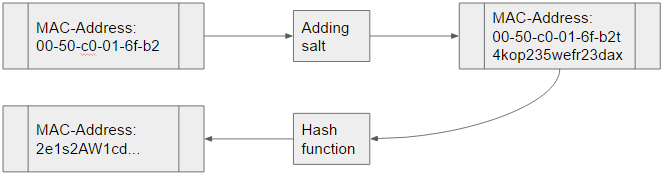
\includegraphics[scale=0.9]{graphics/salt.png}
		\caption{salting and hashing a MAC Address.}
		\label{fig:salt}
	\end{center} 
\end{figure}

\Cref{fig:salt} illustrates how a MAC address is first salted and then hashed.

Java has a hash-method implemented in the object class called \textit{hashCode()}, this may be used for hashing information. When using a hash function, you add a randomly generated string that extends the original message. The generated string is called a salt and makes the hash function more secure.

\subsection*{Hard-coded Passwords}
When communicating with MSE from the intermediate server as well as when communicating with the intermediate server, we are currently using hard-coded passwords. This means that everyone with access to the code can find the log-in information. The information should be given as arguments to the program and hashed such that the log-in can not be seen in the code and cannot be read as plain text in memory. 

%\subsection*{Visibility}
%As of now many parts of the system has a higher degree of visibility than necessary. This makes it possible to use functionality in unexpected ways and possibly cause unintended behaviour. We can decrease the level of visibility by having private and protected classes and methods, which leads to a system that is more resilient towards unexpected usage.
 
\subsection*{Obfuscating Personal Information}
In order to ensure our users personal information, we decided to obfuscate the e-mail addresses. By doing so there will be no way for outsiders to identify people unwilling to have their information stored.

IP addresses are not considered personal information. This is based on the fact that the address changes each time you change access point. By not obfuscating the IP address, applications will be able to see how many people are connected to a given access point. This can be done by identifying the first 16 bits for IPv4 or the first 48 bits for IPv6, also known as the netbits \cite{IPnetworkID}.